\documentclass[aspectratio=169]{ctexbeamer}
% \usetheme{Berkeley}%使用Berkeley主题
\usefonttheme[onlymath]{serif}
\usepackage{amsmath}      % 数学公式支持
\usepackage{xeCJK}
\usepackage{tikz}
\usetikzlibrary{decorations.pathreplacing}%使用大括号
\usetikzlibrary{calligraphy} %calligraphy 书法风格
% \usetikzlibrary{positioning}
\usetikzlibrary{calc}
\usetikzlibrary{backgrounds} %特定的绘图操作置于背景层
\usetikzlibrary{3d}
\usepackage{pgfplots}
\usepgfplotslibrary{fillbetween}
\setCJKmainfont{STKaiti}  % Windows/Linux 系统
\usepackage{caption}  % 或 \usepackage{capt-of}
\begin{document}

% \title[随机事件的概念]{8.1.1 随机事件的概念}%文章标题
\title{高一下期末复习}
\date{2025 年 5 月 15 日}
\begin{frame}{}{}%大标题和小标题的设置与否根据自身需求设定
    \titlepage{}
\end{frame}

% \begin{frame}{大纲}
%   \tableofcontents
% \end{frame}






\begin{frame}[allowframebreaks]{利用斜率判断直线平行}
  \begin{block}{定理}

    设两条直线 \( l_1 \) 和 \( l_2 \) 的斜率分别为 \( k_1 \) 和 \( k_2 \),则:
    \[
    l_1 \parallel l_2 \iff k_1 = k_2 \quad \text{且} \quad b_1 \neq b_2
    \]
    其中 \( b_1 \) 和 \( b_2 \) 分别为两直线在 \( y \)-轴上的截距。
  \end{block}

  \begin{exampleblock}{示例 1}
    判断直线 \( l_1: y = 2x + 3 \) 和 \( l_2: 4x - 2y + 5 = 0 \) 是否平行。
    \begin{enumerate}
      \item 将 \( l_2 \) 化为斜截式:
        \[
        4x - 2y + 5 = 0 \implies y = 2x + \frac{5}{2}
        \]
      \item 比较斜率:
        \[
        k_1 = 2, \quad k_2 = 2 \implies k_1 = k_2
        \]
      \item 比较截距:
        \[
        b_1 = 3, \quad b_2 = \frac{5}{2} \implies b_1 \neq b_2
        \]
      \item 结论:\( l_1 \parallel l_2 \)。
    \end{enumerate}
  \end{exampleblock}
\end{frame}



\begin{frame}{特殊情况:垂直于 \( x \)-轴的直线}
  \begin{block}{判定规则}
    两条直线均垂直于 \( x \)-轴时,若它们的 \( x \)-截距不同,则平行:
    \[
    l_1: x = a_1, \quad l_2: x = a_2 \quad (a_1 \neq a_2) \implies l_1 \parallel l_2
    \]
  \end{block}

  \begin{exampleblock}{示例 2}
    判断直线 \( l_1: x = 2 \) 和 \( l_2: x = -3 \) 是否平行。
    \begin{enumerate}
      \item 两直线斜率均不存在(垂直于 \( x \)-轴)。
      \item \( x \)-截距分别为 \( 2 \) 和 \( -3 \),即 \( a_1 \neq a_2 \)。
      \item 结论:\( l_1 \parallel l_2 \)。
    \end{enumerate}
  \end{exampleblock}
\end{frame}

\begin{frame}[allowframebreaks]{利用直线方程的系数判断平行(一般式)}
  \begin{block}{定理}
    设两条直线的一般式方程为:
    \[
    l_1: A_1x + B_1y + C_1 = 0 \quad \text{和} \quad l_2: A_2x + B_2y + C_2 = 0
    \]
    则两直线平行的充要条件是:
    \[
    \frac{A_1}{A_2} = \frac{B_1}{B_2} \neq \frac{C_1}{C_2}
    \]
    若同时满足 \(\frac{A_1}{A_2} = \frac{B_1}{B_2} = \frac{C_1}{C_2}\),则两直线重合。
  \end{block}

  \begin{exampleblock}{示例1:判断平行}
    判断直线 \( l_1: 2x + 4y - 3 = 0 \) 和 \( l_2: 4x + 8y + 5 = 0 \) 是否平行。
    \begin{enumerate}
      \item 计算系数比例:
        \[
        \frac{A_1}{A_2} = \frac{2}{4} = \frac{1}{2}, \quad \frac{B_1}{B_2} = \frac{4}{8} = \frac{1}{2}, \quad \frac{C_1}{C_2} = \frac{-3}{5}
        \]
      \item 比较比例:
        \[
        \frac{1}{2} = \frac{1}{2} \neq \frac{-3}{5} \implies l_1 \parallel l_2
        \]
    \end{enumerate}
  \end{exampleblock}
\end{frame}



\begin{frame}{示例}
  \begin{exampleblock}{示例2:判断重合}
    判断直线 \( l_1: 3x - y + 2 = 0 \) 和 \( l_2: 6x - 2y + 4 = 0 \) 的关系。
    \begin{enumerate}
      \item 计算系数比例:
        \[
        \frac{A_1}{A_2} = \frac{3}{6} = \frac{1}{2}, \quad \frac{B_1}{B_2} = \frac{-1}{-2} = \frac{1}{2}, \quad \frac{C_1}{C_2} = \frac{2}{4} = \frac{1}{2}
        \]
      \item 比较比例:
        \[
        \frac{1}{2} = \frac{1}{2} = \frac{1}{2} \implies l_1 \text{ 与 } l_2 \text{ 重合}
        \]
    \end{enumerate}
  \end{exampleblock}

\end{frame}

























\begin{frame}{}{}
    求过 $M(3,1)$ 且 与 圆 $(x-1)^2 +y ^2 = 4$ 相切的直线 $l$ 方程.

    \pause
    切线方程为:
    \[
    \boxed{x=3} \quad \text{和} \quad \boxed{3x +4y -13 =0}.
    \]
\end{frame}
\begin{frame}{}{}
    圆 $x^2 + y^2 -2x = 0$ 上点 到直线 $x - y +1 = 0$ 的最小距离为?

    \pause 
    圆心坐标为 $(1,0)$,半径 $r=1$。

    计算圆心到直线 $x - y +1 = 0$ 的距离:
\[
d = \frac{|1 -0 +1|}{\sqrt{1^2 + (-1)^2}} = \frac{2}{\sqrt{2}} = \sqrt{2}
\]

最终答案:
\[
\boxed{\sqrt{2} -1}
\]

\end{frame}

\begin{frame}{}{}
    已知直线 $l_1 : (a-1) x + 2 y +1 = 0 $与 $l_2 :x+ay+3 = 0$ 平行,则 $a = $?

    \pause 

    $2$ 或 $-1$.
\end{frame}

\begin{frame}{}{}
    若直线 $l:mx - m^2 y = 1$ 过点 $P(2,1)$, 则直线$l$的方程为?

    \pause 

    $x-y =1$.
\end{frame}

\begin{frame}{}{}
    若方程 $x^2 +y^2 + ax + 2 ay +2a^2 +a -1 =0$ 表示圆,则 a 的取值范围为?

    \pause

    $(-2,\frac{2}{3})$
\end{frame}
\begin{frame}{}{}
    已知圆 $x^2 +y^2 - 2x +4y -4 = 0$,则过点$P(-3,4)$且与圆相切的切线长为?

    \pause
    $\sqrt{43}.$
\end{frame}





% \section{第七单元}
% 


\begin{frame}{直三棱柱体积与表面积计算}
    \begin{block}{题目}
      直三棱柱底面为直角三角形,直角边分别为 \(3\) 和 \(4\),侧棱长(高)为 \(5\),求体积和表面积。
    \end{block}
  \pause
    \begin{enumerate}
      \item[1.] \textbf{计算底面积}  
        \[
        S_{\text{底}} = \frac{1}{2} \times 3 \times 4 = 6
        \]
      \item[2.] \textbf{计算体积}  
        \[
        V = S_{\text{底}} \times h = 6 \times 5 = 30
        \]
      \item[3.] \textbf{计算底面斜边}  
        \[
        c = \sqrt{3^2 + 4^2} = 5
        \]
      \item[4.] \textbf{计算侧面积与表面积}  
        \[
        S_{\text{侧}} = (3 + 4 + 5) \times 5 = 60, \quad S = 2 \times 6 + 60 = 72
        \]
    \end{enumerate}
  
    \begin{exampleblock}{答案}
      体积:\(\boxed{30}\),表面积:\(\boxed{72}\)
    \end{exampleblock}
  \end{frame}
  
  \begin{frame}{正四棱柱体积与棱长计算}
    \begin{block}{题目}
      正四棱柱底面边长为 \(5\),体积为 \(200\),求侧棱长(高)和表面积。
    \end{block}
  \pause
    \begin{enumerate}
      \item[1.] \textbf{计算底面积}  
        \[
        S_{\text{底}} = 5^2 = 25
        \]
      \item[2.] \textbf{求高}  
        \[
        h = \frac{V}{S_{\text{底}}} = \frac{200}{25} = 8
        \]
      \item[3.] \textbf{计算表面积}  
        \[
        S = 2 \times 25 + 4 \times 5 \times 8 = 50 + 160 = 210
        \]
    \end{enumerate}
  
    \begin{exampleblock}{答案}
      高:\(\boxed{8}\),表面积:\(\boxed{210}\)
    \end{exampleblock}
  \end{frame}
  
  \begin{frame}{长方体空间对角线计算}
    \begin{block}{题目}
      长方体的长、宽、高分别为 \(3\)、\(4\)、\(12\),求空间对角线长度。
    \end{block}
  \pause
    \begin{enumerate}
      \item[1.] \textbf{应用空间对角线公式}  
        \[
        l = \sqrt{a^2 + b^2 + c^2} = \sqrt{3^2 + 4^2 + 12^2} = \sqrt{9 + 16 + 144} = \sqrt{169}
        \]
      \item[2.] \textbf{化简结果}  
        \[
        \sqrt{169} = 13
        \]
    \end{enumerate}
  
    \begin{exampleblock}{答案}
      \(\boxed{13}\)
    \end{exampleblock}
  \end{frame}
  
  \begin{frame}{正六棱柱体积与表面积计算}
    \begin{block}{题目}
      正六棱柱底面边长为 \(2\),高为 \(5\),求体积和表面积。
    \end{block}
  \pause
    \begin{enumerate}
      \item[1.] \textbf{计算底面积}  
        \[
        S_{\text{底}} = \frac{3\sqrt{3}}{2} \times 2^2 = 6\sqrt{3}
        \]
      \item[2.] \textbf{计算体积}  
        \[
        V = 6\sqrt{3} \times 5 = 30\sqrt{3}
        \]
      \item[3.] \textbf{计算侧面积与表面积}  
        \[
        S_{\text{侧}} = 6 \times 2 \times 5 = 60, \quad S = 2 \times 6\sqrt{3} + 60 = 60 + 12\sqrt{3}
        \]
    \end{enumerate}
  
    \begin{exampleblock}{答案}
      体积:\(\boxed{30\sqrt{3}}\),表面积:\(\boxed{60 + 12\sqrt{3}}\)
    \end{exampleblock}
  \end{frame}
  

  \begin{frame}{正六棱柱体积计算(外接圆半径)}
    \begin{block}{题目}
      正六棱柱的高为 \(10\),底面外接圆半径为 \(6\),求体积。
    \end{block}
  \pause
    \begin{enumerate}
      \item[1.] \textbf{确定底面边长}  
        正六边形外接圆半径 \(R = a = 6\)。
      \item[2.] \textbf{计算底面积}  
        \[
        S_{\text{底}} = \frac{3\sqrt{3}}{2} \times 6^2 = 54\sqrt{3}
        \]
      \item[3.] \textbf{计算体积}  
        \[
        V = 54\sqrt{3} \times 10 = 540\sqrt{3}
        \]
    \end{enumerate}
  
    \begin{exampleblock}{答案}
      \(\boxed{540\sqrt{3}}\)
    \end{exampleblock}
  \end{frame}
  

\subsection{棱锥}




\begin{frame}{题目1:表面积、体积计算}
  已知正四棱锥的底面边长为 \(a = 6 \, \text{cm}\),侧棱长为 \(L = 5 \, \text{cm}\),求其体积和表面积。

  \pause

  计算底面中心到边的距离 \(r\):
  \[
  r = \frac{a}{2} = \frac{6}{2} = 3 \, \text{cm}
  \]

  计算斜高 \(l\):
 \[
 l = \sqrt{L^2 - r^2} = \sqrt{5^2 - 3^2} = 4 \, \text{cm}
 \]

 计算四棱锥的高 \(h\):
 \[
 h = \sqrt{l^2 - r^2} = \sqrt{4^2 - 3^2} = \sqrt{7} \, \text{cm}
 \]

 计算体积 \(V\):
 \[
 V = \frac{1}{3} \cdot a^2 \cdot h = \frac{1}{3} \times 6^2 \times \sqrt{7} = 12\sqrt{7} \, \text{cm}^3
 \]

\end{frame}


\begin{frame}{题目2:表面积计算}
  \begin{block}{题目}
      正四棱锥底面边长 \(a = 5 \, \text{cm}\),斜高 \(l = 4 \, \text{cm}\),求其表面积。
  \end{block}
  
  \pause
  
  \begin{alertblock}{解答步骤}
      \begin{enumerate}
          \item 底面面积:\( S_{\text{底}} = a^2 = 5^2 = 25 \, \text{cm}^2 \)
          \item 侧面面积:\( S_{\text{侧}} = \frac{1}{2} a l = \frac{1}{2} \times 5 \times 4 = 10 \, \text{cm}^2 \)
          \item 总表面积:\( S = S_{\text{底}} + 4 S_{\text{侧}} = 25 + 4 \times 10 = 65 \, \text{cm}^2 \)
      \end{enumerate}
  \end{alertblock}
\end{frame}


\begin{frame}{题目3:侧棱长计算}
  \begin{block}{题目}
      已知正四棱锥底面边长 \(a = 6 \, \text{cm}\),高 \(h = 4 \, \text{cm}\),求侧棱长 \(L\)。
  \end{block}
  
  \pause
  
  \begin{alertblock}{解答步骤}
      \begin{enumerate}
          \item 底面中心到边的距离:\( r = \frac{a}{2} = \frac{6}{2} = 3 \, \text{cm} \)
          \item 斜高 :\( l = \sqrt{h^2 + r^2} = 5 \text{cm} \)
          \item $L = \sqrt{l^2 + r^2} = \sqrt{34} \text{cm} $
      \end{enumerate}
  \end{alertblock}
\end{frame}


\begin{frame}{题目4:综合应用}
  \begin{block}{题目}
      正四棱锥表面积为 \(144 \, \text{cm}^2\),底面边长 \(a = 6 \, \text{cm}\),求体积。
  \end{block}
  
  \pause
  
  \begin{alertblock}{解答步骤}
      \begin{enumerate}
          \item 底面面积:\( S_{\text{底}} = a^2 = 6^2 = 36 \, \text{cm}^2 \)
          \item 侧面积总和:\( S_{\text{侧总}} = 144 - 36 = 108 \, \text{cm}^2 \)
          \item 单个侧面面积:\( S_{\text{侧}} = \frac{108}{4} = 27 \, \text{cm}^2 \)
          \item 斜高:\( l = \frac{2 S_{\text{侧}}}{a} = \frac{2 \times 27}{6} = 9 \, \text{cm} \)
          \item 高:\( h = \sqrt{l^2 - \left(\frac{a}{2}\right)^2} = \sqrt{9^2 - 3^2} = 6\sqrt{2} \, \text{cm} \)
          \item 体积:\( V = \frac{1}{3} S_{\text{底}} h = \frac{1}{3} \times 36 \times 6\sqrt{2} = 72\sqrt{2} \, \text{cm}^3 \)
      \end{enumerate}
  \end{alertblock}
\end{frame}




\subsubsection{正三棱锥知识点}


\begin{frame}{正三棱锥结构图}

  \begin{minipage}[t][\textheight][t]{\textwidth}
    \centering
\begin{columns}
    \begin{column}{0.48\textwidth}
    \centering
    \begin{figure}
      \resizebox{!}{3cm}{ % 高度固定为5cm,宽度自动调整
      
% \begin{figure}[H]
    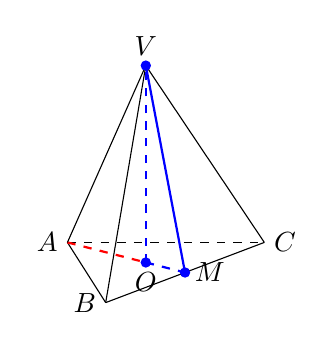
\begin{tikzpicture}[scale=2.5,
        y={(-0.353cm,-0.353cm)}, % 设置 x 轴方向
        x={(1cm,0cm)},            % 设置 y 轴方向
        z={(0cm,1cm)}             % 设置 z 轴方向
    ]%斜二测画法
    % 定义底面正三角形的顶点
    \coordinate (A) at (0,0,0);
    \coordinate (C) at (1,0,0);
    \coordinate (B) at (0.5,{sqrt(3)/2},0);
    
    % 定义顶点 V
    \coordinate (V) at (0.5,{sqrt(3)/6},1);
    
    % 计算底面中心 O
    \coordinate (O) at (0.5,{sqrt(3)/6},0);
    
    % 计算各边中点
    \coordinate (O') at ($(A)!0.5!(C)$);
    \coordinate (M) at ($(C)!0.5!(B)$);
    \coordinate (O''') at ($(B)!0.5!(A)$);
    
    % 绘制底面
    \draw[dashed] (A) -- (C);
    \draw (A) -- (B);
    \draw (C) -- (B);
  
    %%高
    \draw[dashed,red,thick] (A) -- (O);
    \draw[dashed,blue,thick] (O) -- (M);
  
  
    
    % 绘制侧面
    \draw (A) -- (V);
    \draw (C) -- (V);
    \draw (B) -- (V);
    %% 斜高
    \draw[blue,thick] (V) -- (M);
    % 棱锥的高
    \draw[thick,blue,dashed] (O) -- (V); 
    
    % 标记顶点
    \node[left] at (A) {$A$};
    \node[right] at (C) {$C$};
    \node[left] at (B) {$B$};
    \node[above] at (V) {$V$};
    \node[below] at (O) {$O$};
  
    \node[right] at (M) {$M$};
    % 绘制圆点
    \fill[blue] (V) circle (0.75pt);
    \fill[blue] (O) circle (0.75pt);
    \fill[blue] (M) circle (0.75pt);
    \end{tikzpicture}
    % \caption{正三棱锥立体图}
% \end{figure} 
  
      }
      \caption{正三棱锥立体图}
\end{figure}

    \end{column}
    \hfill % 两栏之间的间隔
    \begin{column}{0.48\textwidth}
    \centering
    \begin{figure}
      \resizebox{!}{3cm}{ % 高度固定为5cm,宽度自动调整
      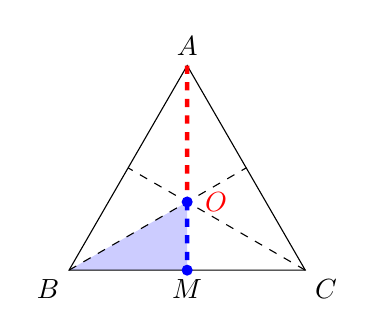
\begin{tikzpicture}[scale=1]
    % 定义正三角形的边长
    \def\sideLength{3}
    % 定义点(按 B、C、A 顺序)
    \coordinate (B) at (0,0);        % 原 A 点改为 B
    \coordinate (C) at (\sideLength,0);  % 原 B 点改为 C
    \coordinate (A) at (\sideLength/2,{sqrt(3)*\sideLength/2}); % 原 C 点改为 A
    
    % 计算 BC 的中点(原 AB 中点改为 BC 中点,H 改为 M)
    \coordinate (M) at ($(B)!0.5!(C)$); % 中点 M 对应新的边 BC
    \coordinate (O) at ($(M)!0.3333!(A)$); % 重心 O(原指向 C,现指向新顶点 A)

    % 填涂区域(保持原逻辑,随顶点变化自动调整)
    \fill[blue!20] (B) -- (O) -- (M) -- cycle; % 顶点改为 B、O、M

    % 绘制正三角形(边改为 B-C-A-B)
    \draw (B) -- (C) -- (A) -- cycle;
    
    % 绘制辅助线(调整指向新顶点)
    \draw[dashed,ultra thick, red] (A) -- (O); % 原 C-O 改为 A-O(红色)
    \draw[dashed,ultra thick,blue] (O) -- (M); % 保持 O-M 不变(蓝色)
    \draw[dashed] (B) -- ($(A)!0.5!(C)$); % 原 A 到 BC 中点,现 B 到 AC 中点
    \draw[dashed] (C) -- ($(A)!0.5!(B)$); % 原 B 到 AC 中点,现 C 到 AB 中点

    % 标记顶点(全部改为新标签)
    \node[below left] at (B) {$B$};  % 原 A 标签改为 B
    \node[below right] at (C) {$C$};  % 原 B 标签改为 C
    \node[above] at (A) {$A$};       % 原 C 标签改为 A
    \node[below] at (M) {$M$}; % 中点 M 标签(原 H 改为 M)
    \node[right=3pt,red] at (O) {$O$}; % 重心 O 标签不变
    \fill[blue] (O) circle (2pt);% 填涂测试点
    \fill[blue] (M) circle (2pt);% 填涂测试点
\end{tikzpicture}
% \captionof{这是一个简单的圆形}  % 添加标题}
      \caption{底面图}
    \end{figure}
    \end{column}
  \end{columns}
  \end{minipage}
  \end{frame}


\subsubsection{正三棱锥}



\begin{frame}{正三棱锥体积计算}
    \begin{block}{题目}
      正三棱锥底面边长为 \(6\),侧棱长为 \(5\),求其体积。
    \end{block}
  
    \pause
    \begin{enumerate}
      \item[1.] \textbf{求底面中心到顶点的距离}  
        底面为正三角形,边长 \(a = 6\),中心到顶点的距离:  
        \[
        d = \frac{\sqrt{3}}{3}a = \frac{\sqrt{3}}{3} \times 6 = 2\sqrt{3}
        \]
  
      \item[2.] \textbf{求三棱锥的高}  
        侧棱长 \(l = 5\),由勾股定理:  
        \[
        h = \sqrt{l^2 - d^2} = \sqrt{5^2 - (2\sqrt{3})^2} = \sqrt{25 - 12} = \sqrt{13}
        \]
  
      \item[3.] \textbf{求底面积}  
        正三角形面积公式:  
        \[
        S = \frac{\sqrt{3}}{4}a^2 = \frac{\sqrt{3}}{4} \times 6^2 = 9\sqrt{3}
        \]
  
      \item[4.] \textbf{计算体积}  
        体积公式 \(V = \frac{1}{3}Sh\):  
        \[
        V = \frac{1}{3} \times 9\sqrt{3} \times \sqrt{13} = 3\sqrt{39}
        \]
    \end{enumerate}
  
  \end{frame}
  
  \begin{frame}{正三棱锥表面积计算}
    \begin{block}{题目}
      正三棱锥底面边长为 \(4\),斜高为 \(3\),求其表面积。
    \end{block}
    \pause
  
    \begin{enumerate}
      \item[1.] \textbf{计算底面积 \(S_{\text{底}}\)}  
        底面为正三角形,边长 \(a = 4\):  
        \[
        S_{\text{底}} = \frac{\sqrt{3}}{4}a^2 = \frac{\sqrt{3}}{4} \times 4^2 = 4\sqrt{3}
        \]
  
      \item[2.] \textbf{计算单个侧面面积 \(S_{\text{侧}}\)}  
        侧面为等腰三角形,底为 \(a = 4\),高为斜高 \(l = 3\):  
        \[
        S_{\text{侧}} = \frac{1}{2} \times a \times l = \frac{1}{2} \times 4 \times 3 = 6
        \]
  
      \item[3.] \textbf{计算总侧面积 \(S_{\text{侧总}}\)}  
        正三棱锥有3个全等的侧面:  
        \[
        S_{\text{侧总}} = 3 \times S_{\text{侧}} = 3 \times 6 = 18
        \]
  
      \item[4.] \textbf{计算表面积 \(S_{\text{表}}\)}  
        表面积等于底面积加总侧面积:  
        \[
        S_{\text{表}} = S_{\text{底}} + S_{\text{侧总}} = 4\sqrt{3} + 18
        \]
    \end{enumerate}

  \end{frame}
  


  \begin{frame}{正三棱锥求高计算}
    \begin{block}{题目}
      正三棱锥体积为 \(16\sqrt{3}\),底面边长为 \(6\),求其高。
    \end{block}
    \pause
    \begin{enumerate}
      \item[1.] \textbf{计算底面积 \(S_{\text{底}}\)}  

        底面为正三角形,边长 \(a = 6\):  
        \[
        S_{\text{底}} = \frac{\sqrt{3}}{4}a^2 = \frac{\sqrt{3}}{4} \times 6^2 = 9\sqrt{3}
        \]
  
      \item[2.] \textbf{利用体积公式反推高 \(h\)}  
      
        体积公式 \(V = \frac{1}{3}S_{\text{底}}h\),变形得:  
        \[
        h = \frac{3V}{S_{\text{底}}} = \frac{3 \times 16\sqrt{3}}{9\sqrt{3}} = \frac{48\sqrt{3}}{9\sqrt{3}} = \frac{16}{3}
        \]
    \end{enumerate}
  
    \begin{exampleblock}{答案}
      \[
      \boxed{\dfrac{16}{3}}
      \]
    \end{exampleblock}
  \end{frame}
  
  \begin{frame}{正三棱锥侧棱长计算}
    \begin{block}{题目}
      正三棱锥高为 \(4\),底面边长为 \(6\),求其侧棱长。
    \end{block}
  \pause
    \begin{enumerate}
      \item[1.] \textbf{计算底面中心到顶点的距离 \(d\)}  
      
        底面为正三角形,边长 \(a = 6\):  
        \[
        d = \frac{\sqrt{3}}{3}a = \frac{\sqrt{3}}{3} \times 6 = 2\sqrt{3}
        \]
  
      \item[2.] \textbf{利用勾股定理求侧棱长 \(l\)}  
      
        高 \(h = 4\),侧棱长、高与底面中心到顶点距离构成直角三角形:  
        \[
        l = \sqrt{h^2 + d^2} = \sqrt{4^2 + (2\sqrt{3})^2} = \sqrt{16 + 12} = \sqrt{28} = 2\sqrt{7}
        \]
    \end{enumerate}
  
    \begin{exampleblock}{答案}
      \[
      \boxed{2\sqrt{7}}
      \]
    \end{exampleblock}
  \end{frame}
  
% 
\subsection{圆柱}
\begin{frame}{圆柱的基本概念}
    \begin{block}{定义}
        圆柱是由两个平行且全等的圆面(底面)和一个连接两底面的曲面(侧面)所围成的几何体。
    \end{block}
    
    \begin{columns}
        \column{0.5\textwidth}
        \begin{exampleblock}{参数}
            \begin{itemize}
                \item 底面半径:\( r \)
                \item 高:\( h \)
                \item 底面面积:\( S_{\text{底}} = \pi r^2 \)
                \item 底面周长:\( C = 2\pi r \)
            \end{itemize}
        \end{exampleblock}
        
        \column{0.5\textwidth}
   
\subsection{圆柱}
\begin{frame}{圆柱的基本概念}
    \begin{block}{定义}
        圆柱是由两个平行且全等的圆面(底面)和一个连接两底面的曲面(侧面)所围成的几何体。
    \end{block}
    
    \begin{columns}
        \column{0.5\textwidth}
        \begin{exampleblock}{参数}
            \begin{itemize}
                \item 底面半径:\( r \)
                \item 高:\( h \)
                \item 底面面积:\( S_{\text{底}} = \pi r^2 \)
                \item 底面周长:\( C = 2\pi r \)
            \end{itemize}
        \end{exampleblock}
        
        \column{0.5\textwidth}
   
\subsection{圆柱}
\begin{frame}{圆柱的基本概念}
    \begin{block}{定义}
        圆柱是由两个平行且全等的圆面(底面)和一个连接两底面的曲面(侧面)所围成的几何体。
    \end{block}
    
    \begin{columns}
        \column{0.5\textwidth}
        \begin{exampleblock}{参数}
            \begin{itemize}
                \item 底面半径:\( r \)
                \item 高:\( h \)
                \item 底面面积:\( S_{\text{底}} = \pi r^2 \)
                \item 底面周长:\( C = 2\pi r \)
            \end{itemize}
        \end{exampleblock}
        
        \column{0.5\textwidth}
   \input{高一下期末复习/tikz/圆柱.tex}

    \end{columns}
\end{frame}



\begin{frame}{表面积与体积公式}
    \begin{block}{核心公式}
        \begin{itemize}
            \item 侧面积:\( S_{\text{侧}} = 2\pi r h \)
            \item 全面积:\( S_{\text{全}} = 2\pi r h + 2\pi r^2 \)
            \item 体积:\( V = \pi r^2 h \)
        \end{itemize}
    \end{block}
    
    \begin{exampleblock}{推导思路}
        \begin{itemize}
            \item 侧面积公式:将侧面展开为矩形,长为底面圆周长 \( 2\pi r \),宽为高 \( h \)
            \item 全面积公式:侧面积加上两个底面积
            \item 体积公式:底面积乘以高
        \end{itemize}
    \end{exampleblock}
\end{frame}

\begin{frame}{圆柱的截面性质}
    \begin{block}{定理}
        圆柱的截面有以下几种情况:
        \begin{enumerate}
            \item 平行于底面的截面:与底面全等的圆
            \item 过轴的截面(轴截面):矩形,长为底面直径 \( 2r \),宽为高 \( h \)
        \end{enumerate}
    \end{block}
    
    \begin{columns}
        \column{0.5\textwidth}
        \begin{exampleblock}{轴截面面积}
            \[
            S_{\text{轴}} = 2r \times h = 2rh
            \]
        \end{exampleblock}
        
        \column{0.5\textwidth}
        \input{高一下期末复习/tikz/圆柱轴截面.tex}
    \end{columns}
\end{frame}





\begin{frame}
    \frametitle{圆柱知识点}
    \begin{itemize}
        \item 圆柱侧面积公式:\( S_{\text{侧}} = 2\pi rh \)
        \item 圆柱表面积公式:\( S_{\text{表}} = 2\pi r(r + h) \)
        \item 圆柱体积公式:\( V = \pi r^2 h \)
    \end{itemize}
\end{frame}



\begin{frame}
    \frametitle{题目1:已知半径和高,求表面积和体积}
    \begin{block}{题目}
        圆柱底面半径为 \(2 \, \text{cm}\),高为 \(5 \, \text{cm}\),求:
        \begin{enumerate}
            \item 侧面积
            \item 表面积
            \item 体积
        \end{enumerate}
    \end{block}
    
    \vspace{0.5cm}
    \pause
    \begin{block}{解答}
        \begin{enumerate}
            \item
            \[
            S_{\text{侧}} = 2\pi \times 2 \times 5 = 20\pi \, \text{cm}^2
            \]
            
            \item 
            \[
            S_{\text{表}} = 2\pi \times 2 \times (2 + 5) = 28\pi \, \text{cm}^2
            \]
            
            \item 
            \[
            V = \pi \times 2^2 \times 5 = 20\pi \, \text{cm}^3
            \]
        \end{enumerate}
    \end{block}
\end{frame}



% 题目2
\begin{frame}
    \frametitle{题目2:已知直径和高,求体积}
    \begin{block}{题目}
        圆柱底面直径为 \(6 \, \text{dm}\),高为 \(4 \, \text{dm}\),求体积。
    \end{block}
    
    \vspace{0.5cm}
    \pause
    \begin{block}{解答}
        首先计算底面半径:
        \[
        r = \frac{d}{2} = \frac{6}{2} = 3 \, \text{dm}
        \]
        
        体积公式:\( V = \pi r^2 h \)
        \[
        V = \pi \times 3^2 \times 4 = 36\pi \, \text{dm}^3
        \]
    \end{block}
\end{frame}

% 题目3
\begin{frame}
    \frametitle{题目3:已知周长和高,求侧面积}
    \begin{block}{题目}
        圆柱底面周长为 \(8\pi \, \text{m}\),高为 \(3 \, \text{m}\),求侧面积。
    \end{block}
    
    \vspace{0.5cm}
    \pause
    
    \begin{block}{解答}
        侧面积公式:\( S_{\text{侧}} = C \times h \)(其中 \(C\) 为底面周长)
        \[
        S_{\text{侧}} = 8\pi \times 3 = 24\pi \, \text{m}^2
        \]
    \end{block}
\end{frame}


% 题目3:立体几何与代数结合
\begin{frame}
    \frametitle{题目4:立体几何与代数结合}
    \begin{block}{题目}
        圆柱的体积为 \(72\pi \, \text{cm}^3\),底面半径与高的比为 \(2:3\),求底面半径和高。
    \end{block}
    \pause
    
    \begin{block}{解析}
        设底面半径为 \(2k\),高为 \(3k\),则体积:
        \[
        V = \pi (2k)^2 \cdot 3k = 12\pi k^3
        \]
        由题可知:
        \[
        12\pi k^3 = 72\pi \implies k^3 = 6 \implies k = \sqrt[3]{6}
        \]
        因此:
        \[
        \text{底面半径} = 2k = 2\sqrt[3]{6} \, \text{cm}, \quad \text{高} = 3k = 3\sqrt[3]{6} \, \text{cm}
        \]
    \end{block}
    
    \begin{alertblock}{答案}
        底面半径:\(2\sqrt[3]{6} \, \text{cm}\),高:\(3\sqrt[3]{6} \, \text{cm}\)
    \end{alertblock}
\end{frame}



% 题目4:最值问题
\begin{frame}[allowframebreaks]
    \frametitle{题目6:最值问题(实际应用)}
    \begin{block}{题目}
        用一张长 \(20\pi \, \text{cm}\)、宽 \(10 \, \text{cm}\) 的矩形纸围成一个圆柱(接口处忽略不计),求围成圆柱的最大体积。
    \end{block}
    
    \begin{block}{解析}
        分两种情况:
        \begin{enumerate}
            \item 以长为底面周长:
            \[
            2\pi r = 20\pi \implies r = 10 \, \text{cm}, \quad h = 10 \, \text{cm}
            \]
            体积:\( V = \pi r^2 h = \pi \times 10^2 \times 10 = 1000\pi \, \text{cm}^3 \)
            
            \item 以宽为底面周长:
            \[
            2\pi r = 10 \implies r = \frac{5}{\pi} \, \text{cm}, \quad h = 20\pi \, \text{cm}
            \]
            体积:\( V = \pi \left(\frac{5}{\pi}\right)^2 \times 20\pi = 500 \, \text{cm}^3 \)
        \end{enumerate}
    \end{block}
    
    \begin{alertblock}{答案}
        最大体积为:\(1000\pi \, \text{cm}^3\)
    \end{alertblock}
\end{frame}

\begin{frame}
    \frametitle{题目7:立体几何与方程结合}
    
    \begin{block}{题目}
        圆柱的表面积为 \(100\pi \, \text{cm}^2\),底面半径与高的和为10 cm。求底面半径。
    \end{block}
    \begin{alertblock}{已知条件}
        \begin{enumerate}
            \item 圆柱表面积 \( S = 100\pi \, \text{cm}^2 \)
            \item 底面半径 \( r \) 与高 \( h \) 的和为10 cm,即 \( r + h = 10 \)
        \end{enumerate}
    \end{alertblock}
    

\end{frame}
\begin{frame}
    \frametitle{解析过程}
    
    \begin{block}{圆柱表面积公式}
        \[
        S = 2\pi r(r + h)
        \]
    \end{block}
    
    \begin{block}{代入已知条件}
        已知 \( S = 100\pi \) 和 \( r + h = 10 \),代入公式得:
        \[
        2\pi r \cdot 10 = 100\pi
        \]
        化简方程:
        \[
        20\pi r = 100\pi
        \]
        两边同时除以 \( 20\pi \):
        \[
        r = \frac{100\pi}{20\pi} = 5 \, \text{cm}
        \]
    \end{block}
\end{frame}

    \end{columns}
\end{frame}



\begin{frame}{表面积与体积公式}
    \begin{block}{核心公式}
        \begin{itemize}
            \item 侧面积:\( S_{\text{侧}} = 2\pi r h \)
            \item 全面积:\( S_{\text{全}} = 2\pi r h + 2\pi r^2 \)
            \item 体积:\( V = \pi r^2 h \)
        \end{itemize}
    \end{block}
    
    \begin{exampleblock}{推导思路}
        \begin{itemize}
            \item 侧面积公式:将侧面展开为矩形,长为底面圆周长 \( 2\pi r \),宽为高 \( h \)
            \item 全面积公式:侧面积加上两个底面积
            \item 体积公式:底面积乘以高
        \end{itemize}
    \end{exampleblock}
\end{frame}

\begin{frame}{圆柱的截面性质}
    \begin{block}{定理}
        圆柱的截面有以下几种情况:
        \begin{enumerate}
            \item 平行于底面的截面:与底面全等的圆
            \item 过轴的截面(轴截面):矩形,长为底面直径 \( 2r \),宽为高 \( h \)
        \end{enumerate}
    \end{block}
    
    \begin{columns}
        \column{0.5\textwidth}
        \begin{exampleblock}{轴截面面积}
            \[
            S_{\text{轴}} = 2r \times h = 2rh
            \]
        \end{exampleblock}
        
        \column{0.5\textwidth}
        \input{高一下期末复习/tikz/圆柱轴截面.tex}
    \end{columns}
\end{frame}





\begin{frame}
    \frametitle{圆柱知识点}
    \begin{itemize}
        \item 圆柱侧面积公式:\( S_{\text{侧}} = 2\pi rh \)
        \item 圆柱表面积公式:\( S_{\text{表}} = 2\pi r(r + h) \)
        \item 圆柱体积公式:\( V = \pi r^2 h \)
    \end{itemize}
\end{frame}



\begin{frame}
    \frametitle{题目1:已知半径和高,求表面积和体积}
    \begin{block}{题目}
        圆柱底面半径为 \(2 \, \text{cm}\),高为 \(5 \, \text{cm}\),求:
        \begin{enumerate}
            \item 侧面积
            \item 表面积
            \item 体积
        \end{enumerate}
    \end{block}
    
    \vspace{0.5cm}
    \pause
    \begin{block}{解答}
        \begin{enumerate}
            \item
            \[
            S_{\text{侧}} = 2\pi \times 2 \times 5 = 20\pi \, \text{cm}^2
            \]
            
            \item 
            \[
            S_{\text{表}} = 2\pi \times 2 \times (2 + 5) = 28\pi \, \text{cm}^2
            \]
            
            \item 
            \[
            V = \pi \times 2^2 \times 5 = 20\pi \, \text{cm}^3
            \]
        \end{enumerate}
    \end{block}
\end{frame}



% 题目2
\begin{frame}
    \frametitle{题目2:已知直径和高,求体积}
    \begin{block}{题目}
        圆柱底面直径为 \(6 \, \text{dm}\),高为 \(4 \, \text{dm}\),求体积。
    \end{block}
    
    \vspace{0.5cm}
    \pause
    \begin{block}{解答}
        首先计算底面半径:
        \[
        r = \frac{d}{2} = \frac{6}{2} = 3 \, \text{dm}
        \]
        
        体积公式:\( V = \pi r^2 h \)
        \[
        V = \pi \times 3^2 \times 4 = 36\pi \, \text{dm}^3
        \]
    \end{block}
\end{frame}

% 题目3
\begin{frame}
    \frametitle{题目3:已知周长和高,求侧面积}
    \begin{block}{题目}
        圆柱底面周长为 \(8\pi \, \text{m}\),高为 \(3 \, \text{m}\),求侧面积。
    \end{block}
    
    \vspace{0.5cm}
    \pause
    
    \begin{block}{解答}
        侧面积公式:\( S_{\text{侧}} = C \times h \)(其中 \(C\) 为底面周长)
        \[
        S_{\text{侧}} = 8\pi \times 3 = 24\pi \, \text{m}^2
        \]
    \end{block}
\end{frame}


% 题目3:立体几何与代数结合
\begin{frame}
    \frametitle{题目4:立体几何与代数结合}
    \begin{block}{题目}
        圆柱的体积为 \(72\pi \, \text{cm}^3\),底面半径与高的比为 \(2:3\),求底面半径和高。
    \end{block}
    \pause
    
    \begin{block}{解析}
        设底面半径为 \(2k\),高为 \(3k\),则体积:
        \[
        V = \pi (2k)^2 \cdot 3k = 12\pi k^3
        \]
        由题可知:
        \[
        12\pi k^3 = 72\pi \implies k^3 = 6 \implies k = \sqrt[3]{6}
        \]
        因此:
        \[
        \text{底面半径} = 2k = 2\sqrt[3]{6} \, \text{cm}, \quad \text{高} = 3k = 3\sqrt[3]{6} \, \text{cm}
        \]
    \end{block}
    
    \begin{alertblock}{答案}
        底面半径:\(2\sqrt[3]{6} \, \text{cm}\),高:\(3\sqrt[3]{6} \, \text{cm}\)
    \end{alertblock}
\end{frame}



% 题目4:最值问题
\begin{frame}[allowframebreaks]
    \frametitle{题目6:最值问题(实际应用)}
    \begin{block}{题目}
        用一张长 \(20\pi \, \text{cm}\)、宽 \(10 \, \text{cm}\) 的矩形纸围成一个圆柱(接口处忽略不计),求围成圆柱的最大体积。
    \end{block}
    
    \begin{block}{解析}
        分两种情况:
        \begin{enumerate}
            \item 以长为底面周长:
            \[
            2\pi r = 20\pi \implies r = 10 \, \text{cm}, \quad h = 10 \, \text{cm}
            \]
            体积:\( V = \pi r^2 h = \pi \times 10^2 \times 10 = 1000\pi \, \text{cm}^3 \)
            
            \item 以宽为底面周长:
            \[
            2\pi r = 10 \implies r = \frac{5}{\pi} \, \text{cm}, \quad h = 20\pi \, \text{cm}
            \]
            体积:\( V = \pi \left(\frac{5}{\pi}\right)^2 \times 20\pi = 500 \, \text{cm}^3 \)
        \end{enumerate}
    \end{block}
    
    \begin{alertblock}{答案}
        最大体积为:\(1000\pi \, \text{cm}^3\)
    \end{alertblock}
\end{frame}

\begin{frame}
    \frametitle{题目7:立体几何与方程结合}
    
    \begin{block}{题目}
        圆柱的表面积为 \(100\pi \, \text{cm}^2\),底面半径与高的和为10 cm。求底面半径。
    \end{block}
    \begin{alertblock}{已知条件}
        \begin{enumerate}
            \item 圆柱表面积 \( S = 100\pi \, \text{cm}^2 \)
            \item 底面半径 \( r \) 与高 \( h \) 的和为10 cm,即 \( r + h = 10 \)
        \end{enumerate}
    \end{alertblock}
    

\end{frame}
\begin{frame}
    \frametitle{解析过程}
    
    \begin{block}{圆柱表面积公式}
        \[
        S = 2\pi r(r + h)
        \]
    \end{block}
    
    \begin{block}{代入已知条件}
        已知 \( S = 100\pi \) 和 \( r + h = 10 \),代入公式得:
        \[
        2\pi r \cdot 10 = 100\pi
        \]
        化简方程:
        \[
        20\pi r = 100\pi
        \]
        两边同时除以 \( 20\pi \):
        \[
        r = \frac{100\pi}{20\pi} = 5 \, \text{cm}
        \]
    \end{block}
\end{frame}

    \end{columns}
\end{frame}



\begin{frame}{表面积与体积公式}
    \begin{block}{核心公式}
        \begin{itemize}
            \item 侧面积:\( S_{\text{侧}} = 2\pi r h \)
            \item 全面积:\( S_{\text{全}} = 2\pi r h + 2\pi r^2 \)
            \item 体积:\( V = \pi r^2 h \)
        \end{itemize}
    \end{block}
    
    \begin{exampleblock}{推导思路}
        \begin{itemize}
            \item 侧面积公式:将侧面展开为矩形,长为底面圆周长 \( 2\pi r \),宽为高 \( h \)
            \item 全面积公式:侧面积加上两个底面积
            \item 体积公式:底面积乘以高
        \end{itemize}
    \end{exampleblock}
\end{frame}

\begin{frame}{圆柱的截面性质}
    \begin{block}{定理}
        圆柱的截面有以下几种情况:
        \begin{enumerate}
            \item 平行于底面的截面:与底面全等的圆
            \item 过轴的截面(轴截面):矩形,长为底面直径 \( 2r \),宽为高 \( h \)
        \end{enumerate}
    \end{block}
    
    \begin{columns}
        \column{0.5\textwidth}
        \begin{exampleblock}{轴截面面积}
            \[
            S_{\text{轴}} = 2r \times h = 2rh
            \]
        \end{exampleblock}
        
        \column{0.5\textwidth}
        \input{高一下期末复习/tikz/圆柱轴截面.tex}
    \end{columns}
\end{frame}





\begin{frame}
    \frametitle{圆柱知识点}
    \begin{itemize}
        \item 圆柱侧面积公式:\( S_{\text{侧}} = 2\pi rh \)
        \item 圆柱表面积公式:\( S_{\text{表}} = 2\pi r(r + h) \)
        \item 圆柱体积公式:\( V = \pi r^2 h \)
    \end{itemize}
\end{frame}



\begin{frame}
    \frametitle{题目1:已知半径和高,求表面积和体积}
    \begin{block}{题目}
        圆柱底面半径为 \(2 \, \text{cm}\),高为 \(5 \, \text{cm}\),求:
        \begin{enumerate}
            \item 侧面积
            \item 表面积
            \item 体积
        \end{enumerate}
    \end{block}
    
    \vspace{0.5cm}
    \pause
    \begin{block}{解答}
        \begin{enumerate}
            \item
            \[
            S_{\text{侧}} = 2\pi \times 2 \times 5 = 20\pi \, \text{cm}^2
            \]
            
            \item 
            \[
            S_{\text{表}} = 2\pi \times 2 \times (2 + 5) = 28\pi \, \text{cm}^2
            \]
            
            \item 
            \[
            V = \pi \times 2^2 \times 5 = 20\pi \, \text{cm}^3
            \]
        \end{enumerate}
    \end{block}
\end{frame}



% 题目2
\begin{frame}
    \frametitle{题目2:已知直径和高,求体积}
    \begin{block}{题目}
        圆柱底面直径为 \(6 \, \text{dm}\),高为 \(4 \, \text{dm}\),求体积。
    \end{block}
    
    \vspace{0.5cm}
    \pause
    \begin{block}{解答}
        首先计算底面半径:
        \[
        r = \frac{d}{2} = \frac{6}{2} = 3 \, \text{dm}
        \]
        
        体积公式:\( V = \pi r^2 h \)
        \[
        V = \pi \times 3^2 \times 4 = 36\pi \, \text{dm}^3
        \]
    \end{block}
\end{frame}

% 题目3
\begin{frame}
    \frametitle{题目3:已知周长和高,求侧面积}
    \begin{block}{题目}
        圆柱底面周长为 \(8\pi \, \text{m}\),高为 \(3 \, \text{m}\),求侧面积。
    \end{block}
    
    \vspace{0.5cm}
    \pause
    
    \begin{block}{解答}
        侧面积公式:\( S_{\text{侧}} = C \times h \)(其中 \(C\) 为底面周长)
        \[
        S_{\text{侧}} = 8\pi \times 3 = 24\pi \, \text{m}^2
        \]
    \end{block}
\end{frame}


% 题目3:立体几何与代数结合
\begin{frame}
    \frametitle{题目4:立体几何与代数结合}
    \begin{block}{题目}
        圆柱的体积为 \(72\pi \, \text{cm}^3\),底面半径与高的比为 \(2:3\),求底面半径和高。
    \end{block}
    \pause
    
    \begin{block}{解析}
        设底面半径为 \(2k\),高为 \(3k\),则体积:
        \[
        V = \pi (2k)^2 \cdot 3k = 12\pi k^3
        \]
        由题可知:
        \[
        12\pi k^3 = 72\pi \implies k^3 = 6 \implies k = \sqrt[3]{6}
        \]
        因此:
        \[
        \text{底面半径} = 2k = 2\sqrt[3]{6} \, \text{cm}, \quad \text{高} = 3k = 3\sqrt[3]{6} \, \text{cm}
        \]
    \end{block}
    
    \begin{alertblock}{答案}
        底面半径:\(2\sqrt[3]{6} \, \text{cm}\),高:\(3\sqrt[3]{6} \, \text{cm}\)
    \end{alertblock}
\end{frame}



% 题目4:最值问题
\begin{frame}[allowframebreaks]
    \frametitle{题目6:最值问题(实际应用)}
    \begin{block}{题目}
        用一张长 \(20\pi \, \text{cm}\)、宽 \(10 \, \text{cm}\) 的矩形纸围成一个圆柱(接口处忽略不计),求围成圆柱的最大体积。
    \end{block}
    
    \begin{block}{解析}
        分两种情况:
        \begin{enumerate}
            \item 以长为底面周长:
            \[
            2\pi r = 20\pi \implies r = 10 \, \text{cm}, \quad h = 10 \, \text{cm}
            \]
            体积:\( V = \pi r^2 h = \pi \times 10^2 \times 10 = 1000\pi \, \text{cm}^3 \)
            
            \item 以宽为底面周长:
            \[
            2\pi r = 10 \implies r = \frac{5}{\pi} \, \text{cm}, \quad h = 20\pi \, \text{cm}
            \]
            体积:\( V = \pi \left(\frac{5}{\pi}\right)^2 \times 20\pi = 500 \, \text{cm}^3 \)
        \end{enumerate}
    \end{block}
    
    \begin{alertblock}{答案}
        最大体积为:\(1000\pi \, \text{cm}^3\)
    \end{alertblock}
\end{frame}

\begin{frame}
    \frametitle{题目7:立体几何与方程结合}
    
    \begin{block}{题目}
        圆柱的表面积为 \(100\pi \, \text{cm}^2\),底面半径与高的和为10 cm。求底面半径。
    \end{block}
    \begin{alertblock}{已知条件}
        \begin{enumerate}
            \item 圆柱表面积 \( S = 100\pi \, \text{cm}^2 \)
            \item 底面半径 \( r \) 与高 \( h \) 的和为10 cm,即 \( r + h = 10 \)
        \end{enumerate}
    \end{alertblock}
    

\end{frame}
\begin{frame}
    \frametitle{解析过程}
    
    \begin{block}{圆柱表面积公式}
        \[
        S = 2\pi r(r + h)
        \]
    \end{block}
    
    \begin{block}{代入已知条件}
        已知 \( S = 100\pi \) 和 \( r + h = 10 \),代入公式得:
        \[
        2\pi r \cdot 10 = 100\pi
        \]
        化简方程:
        \[
        20\pi r = 100\pi
        \]
        两边同时除以 \( 20\pi \):
        \[
        r = \frac{100\pi}{20\pi} = 5 \, \text{cm}
        \]
    \end{block}
\end{frame}
% 
\subsection{圆锥}
\begin{frame}
    \frametitle{圆锥知识点}
    \begin{itemize}
        \item 圆锥母线长公式:\( l = \sqrt{r^2 + h^2} \)
        \item 圆锥侧面积公式:\( S_{\text{侧}} = \pi r l \)
        \item 圆锥表面积公式:\( S_{\text{表}} = \pi r(r + l) \)
        \item 圆锥体积公式:\( V = \frac{1}{3}\pi r^2 h \)
    \end{itemize}
    
    \vspace{0.5cm}
    
    \begin{columns}
        \column{0.5\textwidth}
        \begin{block}{符号说明}
            \begin{itemize}
                \item \( r \): 底面半径
                \item \( h \): 高
                \item \( l \): 母线长
            \end{itemize}
        \end{block}
        
        \column{0.5\textwidth}
        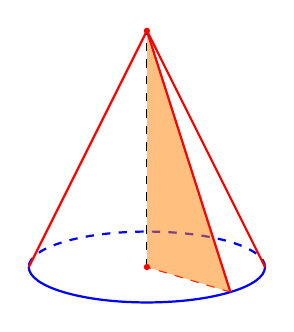
\begin{tikzpicture}[scale=1.5,
            y={(0cm,-0.3cm)}, % 设置 x 轴方向
            x={(1cm,0cm)},            % 设置 y 轴方向
            z={(0cm,1cm)}             % 设置 z 轴方向
        ]
            % 定义圆柱的参数
            \def\radius{1} % 圆锥底面半径
            \def\height{2} % 圆锥的高度
            % 一些坐标
            \coordinate (O') at (0,0,\height);
            \coordinate (O) at (0,0,0);
            %上圆上一点
            \coordinate (A') at ({\radius*sqrt(2)/2},{\radius*sqrt(2)/2},\height);
            %下圆上一点
            \coordinate (A) at ({\radius*sqrt(2)/2},{\radius*sqrt(2)/2},0);
                % 底面半径
                \draw[thin,dashed,red] (A) -- (O);
                % 绘制底面圆
                \begin{scope}
                    \draw [blue,thick,dashed] (\radius,0,0) arc (0:-180:\radius) ;
                    \draw [blue,thick] (\radius,0,0) arc (0:180:\radius) ;
        
                \end{scope}
                \fill[orange,opacity=0.5] (A) -- (O) -- (O') -- cycle;
                % 绘制母线
                \begin{scope}
                    \draw[thick,red] (\radius,0,0) -- (O');
                    \draw[thick,red] (-\radius,0,0) -- (O');
                    \draw[thick,red] (A) -- (O');
                \end{scope}
                
        
                % 绘制高线
                \begin{scope}
                    \draw[thin,dashed] (0,0,0) -- (0,0,\height);
                    \fill[red] (0,0,0) circle (0.75pt);  % 绘制一个点测试一下 
                    \fill[red] (0,0,\height) circle (0.75pt);  % 绘制一个点测试一下 
                \end{scope}
        \end{tikzpicture}
    \end{columns}
\end{frame}



% 幻灯片1:题目1
\begin{frame}
    \frametitle{基础计算题 - 题目1}
    \begin{block}{题目}
        圆锥底面半径为4cm,高为3cm,求其侧面积、表面积和体积。
    \end{block}
    \pause
    
    \begin{block}{解析}
        1. 计算母线长:
        \[
        l = \sqrt{r^2 + h^2} = \sqrt{4^2 + 3^2} = 5 \, \text{cm}
        \]
        2. 
        \(
        S_{\text{侧}} = \pi r l = \pi \times 4 \times 5 = 20\pi \, \text{cm}^2
        \)\\
        3. 
        \(
        S_{\text{表}} = S_{\text{侧}} + \pi r^2 = 20\pi + \pi \times 4^2 = 36\pi \, \text{cm}^2
        \)\\
        4. 体积公式:
        \[
        V = \frac{1}{3} \pi r^2 h = \frac{1}{3} \pi \times 4^2 \times 3 = 16\pi \, \text{cm}^3
        \]
    \end{block}
    
    \begin{alertblock}{\small 答案}
        \small
        侧面积:\(20\pi \, \text{cm}^2\),表面积:\(36\pi \, \text{cm}^2\),体积:\(16\pi \, \text{cm}^3\)
    \end{alertblock}
\end{frame}

% 幻灯片2:题目2
\begin{frame}
    \frametitle{基础计算题 - 题目2}
    \begin{block}{题目}
        圆锥底面直径为6dm,母线长为8dm,求其表面积。
    \end{block}
    \pause
    
    \begin{block}{解析}
        1. 计算底面半径:
        \[
        r = \frac{d}{2} = \frac{6}{2} = 3 \, \text{dm}
        \]
        2. 侧面积公式:
        \(
        S_{\text{侧}} = \pi r l = \pi \times 3 \times 8 = 24\pi \, \text{dm}^2
        \)\\
        3. 底面积公式:
        \(
        S_{\text{底}} = \pi r^2 = \pi \times 3^2 = 9\pi \, \text{dm}^2
        \)\\
        4. 表面积公式:
        \(
        S_{\text{表}} = S_{\text{侧}} + S_{\text{底}} = 24\pi + 9\pi = 33\pi \, \text{dm}^2
        \)
    \end{block}
    
    \begin{alertblock}{答案}
        表面积:\(33\pi \, \text{dm}^2\)
    \end{alertblock}
\end{frame}

% 幻灯片3:题目3
\begin{frame}
    \frametitle{基础计算题 - 题目3}
    \begin{block}{题目}
        圆锥底面周长为\(10\pi\)m,体积为\(\frac{25}{3}\pi\)m³,求其高。
    \end{block}
    \pause
    
    \begin{block}{解析}
        1. 计算底面半径:
        \[
        C = 2\pi r \implies r = \frac{C}{2\pi} = \frac{10\pi}{2\pi} = 5 \, \text{m}
        \]
        2. 体积公式:
        \[
        V = \frac{1}{3} \pi r^2 h \implies \frac{25}{3}\pi = \frac{1}{3} \pi \times 5^2 \times h
        \]
        3. 解方程:
        \[
        \frac{25}{3}\pi = \frac{25}{3}\pi h \implies h = 1 \, \text{m}
        \]
    \end{block}
    
    \begin{alertblock}{答案}
        高:\(1 \, \text{m}\)
    \end{alertblock}
\end{frame}


\begin{frame}
    \frametitle{圆锥表面积计算- 题目4}
    
    \begin{block}{题目}
        一个圆锥的底面半径为 \(6 \, \text{cm}\),高为 \(8 \, \text{cm}\),求它的表面积(结果保留 \(\pi\))。
    \end{block}
    

\end{frame}
\begin{frame}

    \begin{block}{解析}
        \begin{enumerate}
            \item 计算母线长 \( l \):
            \[
            l = \sqrt{r^2 + h^2} = \sqrt{6^2 + 8^2} = \sqrt{100} = 10 \, \text{cm}
            \]
            
            \item 计算侧面积 \( S_{\text{侧}} \):
            \[
            S_{\text{侧}} = \pi r l = \pi \times 6 \times 10 = 60\pi \, \text{cm}^2
            \]
            
            \item 计算底面积 \( S_{\text{底}} \):
            \[
            S_{\text{底}} = \pi r^2 = \pi \times 6^2 = 36\pi \, \text{cm}^2
            \]
            
            \item 计算表面积 \( S_{\text{表}} \):
            \[
            S_{\text{表}} = S_{\text{侧}} + S_{\text{底}} = 60\pi + 36\pi = 96\pi \, \text{cm}^2
            \]
        \end{enumerate}
    \end{block}

    \begin{alertblock}{答案}
        圆锥的表面积为 \(\boxed{96\pi \, \text{cm}^2}\)。
    \end{alertblock}
\end{frame}



% 题目5
\begin{frame}{展开图相关(题目5)}
    \begin{block}{题目}
    圆锥侧面展开图是圆心角216°的扇形,底面半径5cm,求侧面积。
    \end{block}
    \pause
    
    \begin{align*}
    \text{底面周长} &= 2\pi r = 10\pi \\
    \text{扇形弧长} &= \frac{216^\circ}{360^\circ} \times 2\pi l = 10\pi \\
    \Rightarrow l &= \frac{10\pi \times 180^\circ}{216^\circ \pi} = \frac{125}{3}\text{cm} \\
    S_{\text{侧}} &= \pi r l = \pi \times 5 \times \frac{25}{3} = \frac{125}{3}\pi \,\text{cm}^2
    \end{align*}

    \end{frame}



% 题目6
\begin{frame}{展开图相关(题目6)}
    \begin{block}{题目}
    圆锥侧面展开图是半圆形,母线长10cm,求侧面积。
    \end{block}
    
    \pause

    \begin{equation*}
    \begin{cases}
    \text{半圆周长} = \pi l = 10\pi \\
    \text{底面周长} = 2\pi r = 10\pi \Rightarrow r = 5\text{cm} \\
    S_{\text{侧}} = \pi r l = \pi \times 5 \times 10 = 50\pi \,\text{cm}^2
    \end{cases}
    \end{equation*}
    \end{frame}



    % 题目7
\begin{frame}{逆向计算参数(题目7)}
    \begin{block}{题目}
    侧面积30$\pi$ cm²,底面半径4cm,求母线长。
    \end{block}
    \pause
    
    \begin{align*}
    S_{\text{侧}} &= \pi r l \\
    30\pi &= \pi \times 4 \times l \\
    l &= \frac{30\pi}{4\pi} = \frac{15}{2}\,\text{cm} \\
    \end{align*}
    

    \end{frame}
    
    % 题目8
    \begin{frame}{逆向计算参数(题目8)}
    \begin{block}{题目}
    侧面积80$\pi$ cm²,母线长10cm,求底面半径。
    \end{block}
    \pause
    
    $$
    \begin{aligned}
    S_{\text{侧}} &= \pi r l \\
    80\pi &= \pi \times r \times 10 \\
    r &= \frac{80\pi}{10\pi} = 8\text{cm}
    \end{aligned}
    $$
    
   
    \end{frame}
% \subsection{指数幂}
\subsubsection{整数指数幂}
\begin{frame}{1. 整数指数幂的定义}
    \begin{block}{正整数指数幂}
        设 \( a \in \mathbb{R} \),\( n \in \mathbb{N}^* \),则:
        \[
        a^n = \underbrace{a \times a \times \cdots \times a}_{n\text{个}}
        \]
        \vspace{0.5cm}
        \textbf{示例}:\( 2^3 = 8 \), \( (-3)^2 = 9 \)
    \end{block}

    \begin{block}{零指数幂与负整数指数幂}
        \[
        a^0 = 1 \quad (a \neq 0), \quad a^{-n} = \frac{1}{a^n} \quad (a \neq 0, n \in \mathbb{N}^*)
        \]
        \vspace{0.5cm}
        \textbf{示例}:\( 5^0 = 1 \), \( 2^{-3} = \frac{1}{8} \)
    \end{block}
\end{frame}

\begin{frame}{2. 整数指数幂的运算性质}
    \begin{block}{运算公式}
        设 \( a, b \in \mathbb{R} \setminus \{0\} \),\( m, n \in \mathbb{Z} \),则:
        \[
        \begin{aligned}
        &(1)\ a^m \cdot a^n = a^{m+n} \\
        &(2)\ (a^m)^n = a^{mn} \\
        &(3)\ (ab)^n = a^n b^n \\
        &(4)\ \frac{a^m}{a^n} = a^{m-n} \quad (a \neq 0)
        \end{aligned}
        \]
    \end{block}

    \begin{exampleblock}{例题}
        化简:\( (2^3 \cdot 2^{-5}) \div 2^{-2} \)
        \[
        \text{解:原式} = 2^{3-5} \div 2^{-2} = 2^{-2} \div 2^{-2} = 2^0 = 1
        \]
    \end{exampleblock}
\end{frame}



% 第二部分:分数指数幂
\subsubsection{分数指数幂}
\begin{frame}{1. 根式与分数指数幂的互化}
    \begin{block}{$n$次根式定义}
        若 \( x^n = a \)(\( n \geq 2, n \in \mathbb{N}^* \)),则 \( x \) 称为 \( a \) 的$n$次根:
        \[
            x = \sqrt[n]{a} \quad 
            \begin{cases} 
            \text{当 } n \text{ 为奇数时,} a \in \mathbb{R}; \\
            \text{当 } n \text{ 为偶数时,} a \geq 0.
            \end{cases}
        \]
    \end{block}

    \begin{block}{分数指数幂公式}
        \[
        a^{\frac{m}{n}} = \sqrt[n]{a^m} = (\sqrt[n]{a})^m \quad (a > 0, m, n \in \mathbb{N}^*, n > 1)
        \]
        \vspace{0.5cm}
        \textbf{示例}:\( 8^{\frac{2}{3}} = \sqrt[3]{8^2} = 4 \), \( 16^{-\frac{3}{4}} = \frac{1}{\sqrt[4]{16^3}} = \frac{1}{8} \)
    \end{block}
\end{frame}

\begin{frame}{2. 分数指数幂的运算性质}
    \begin{block}{与整数指数幂一致的运算律}
        设 \( a, b > 0 \),\( s, t \in \mathbb{Q} \),则:
        \[
        \begin{aligned}
        &(1)\ a^s \cdot a^t = a^{s+t} \\
        &(2)\ (a^s)^t = a^{st} \\
        &(3)\ (ab)^s = a^s b^s
        \end{aligned}
        \]
    \end{block}

    \begin{exampleblock}{例题}
        计算:\( 4^{\frac{1}{2}} \cdot 8^{\frac{1}{3}} \)
        \[
        \text{解:} \ 4^{\frac{1}{2}} = 2, \ 8^{\frac{1}{3}} = 2 \implies \text{原式} = 2 \times 2 = 4
        \]
    \end{exampleblock}
\end{frame}







% 第三部分:无理数指数幂


\subsubsection{实数指数幂}
\begin{frame}{实数指数幂的统一运算}
    \begin{block}{运算性质的延拓}
        对任意 \( a, b > 0 \),\( s, t \in \mathbb{R} \),以下性质成立:
        \[
        \begin{aligned}
        &(1)\ a^s \cdot a^t = a^{s+t} \\
        &(2)\ (a^s)^t = a^{st} \\
        &(3)\ (ab)^s = a^s b^s
        \end{aligned}
        \]
    \end{block}

    \begin{exampleblock}{例题}
        化简:\( (a^{\sqrt{2}} \cdot a^{\pi})^{\frac{1}{\sqrt{2}+\pi}} \)
        \[
        \text{解:原式} = a^{(\sqrt{2}+\pi)\cdot \frac{1}{\sqrt{2}+\pi}}  = a^1 = a
        \]
    \end{exampleblock}
\end{frame}


\begin{frame}{一、直接计算(每题5分)}
    \begin{enumerate}
        \item 计算:\( 16^{\frac{3}{4}} \)
        \item 计算:\( 27^{-\frac{2}{3}} \)
        \item 计算:\( \left( \frac{16}{81} \right)^{-\frac{3}{4}} \)
        \item 计算:\( 4^{\sqrt{2}} \cdot 2^{1-2\sqrt{2}} \)
    \end{enumerate}
    
    \pause % 暂停后显示答案
    \begin{block}{答案}
        \[
        \begin{aligned}
        &1.\ 8 \quad \quad \quad \\
        &2.\ \frac{1}{9} \\
        &3.\ \frac{27}{8} \quad \\
        & 4.\ 2
        \end{aligned}
        \]
    \end{block}
\end{frame}








\subsection{指数函数}
\begin{frame}{指数函数的定义}
    \begin{block}{定义}
        形如 \( f(x) = a^x \) 的函数称为指数函数,其中底数 \( a > 0 \) 且 \( a \neq 1 \),自变量 \( x \) 是实数。
    \end{block}
    
    \begin{itemize}
        \item 当 \( a > 1 \) 时,函数单调递增
        \item 当 \( 0 < a < 1 \) 时,函数单调递减
        \item 特殊情况:自然指数函数 \( e^x \)(\( e \approx 2.71828 \))
    \end{itemize}
  \end{frame}
  
  
  
  \begin{frame}{指数函数的图像}
    \begin{columns}
        \begin{column}{0.5\textwidth}
            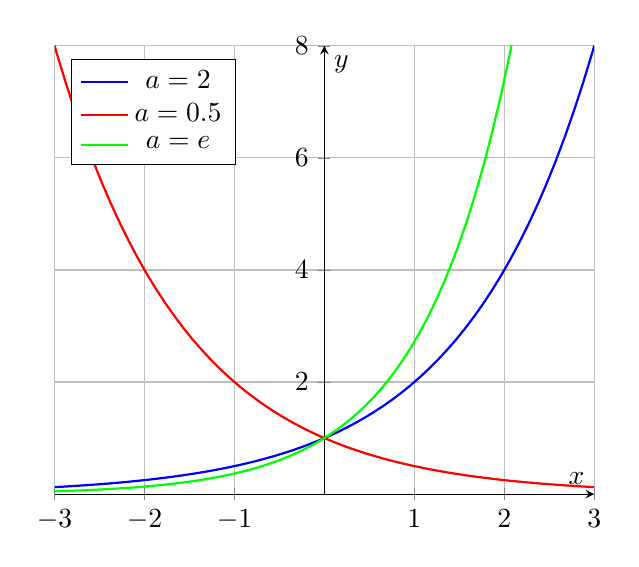
\begin{tikzpicture}
                \begin{axis}[
                    xmin=-3, xmax=3,
                    ymin=0, ymax=8,
                    axis lines=middle,
                    xlabel=$x$, ylabel=$y$,
                    grid=both,
                    samples=100,
                    legend pos=north west
                ]
                \addplot[blue, thick] {2^x};
                \addlegendentry{$a=2$};
                \addplot[red, thick] {(1/2)^x};
                \addlegendentry{$a=0.5$};
                \addplot[green, thick] {exp(x)};
                \addlegendentry{$a=e$};
                \end{axis}
            \end{tikzpicture}
        \end{column}
        \begin{column}{0.5\textwidth}
            \begin{itemize}
                \item 所有指数函数过点 \((0,1)\)
                \item \( a > 1 \) 时,函数图像向上增长
                \item \( 0 < a < 1 \) 时,函数图像向下趋近于 x 轴
                \item $x$ 轴是水平渐近线,也就是函数的值只能无限接近$0$.
                % \item 值域是$(0,+\infty)$
                % \item 定义域是$\mathbf{R}$,即 \( (-\infty, +\infty)\)
            \end{itemize}
        \end{column}
    \end{columns}
  \end{frame}
  
  
  \begin{frame}{定义域和值域}
    \begin{block}{定义域}
        指数函数 \( f(x) = a^x \) 的定义域是全体实数,即 \( (-\infty, +\infty) \)。
    \end{block}
    
    \begin{block}{值域}
        指数函数的值域是正实数集,即 \( (0, +\infty) \)。
    \end{block}
    
    \begin{center}
        \begin{tikzpicture}
            \draw[->] (-3,0) -- (3,0) node[right] {$x$};
            \draw[->] (0,-0.5) -- (0,3) node[above] {$y$};
            \draw[blue, thick, domain=-3:3] plot (\x, {exp(\x)/5});
            \draw[dashed] (-3,0) -- (3,0);
            % \node at (0,1.5) {值域:$(0,+\infty)$};
            % \node at (-2,0.2) {定义域:$(-\infty,+\infty)$};
        \end{tikzpicture}
    \end{center}
  \end{frame}
  
  
  \begin{frame}{单调性}
    \begin{columns}
        \begin{column}{0.5\textwidth}
            \textbf{当 \( a > 1 \) 时:}
            \begin{itemize}
                \item 函数严格递增
                % \item 导数 \( f'(x) = a^x \ln a > 0 \)
                \item 示例:\( f(x) = 2^x \)
            \end{itemize}
            
            \begin{tikzpicture}[scale=0.7]
                \begin{axis}[
                    xmin=-2, xmax=2,
                    ymin=0, ymax=4,
                    axis lines=middle,
                    samples=50,
                    xtick={-2,-1,0,1,2},
                    ytick={1,2,4}
                ]
                \addplot[blue, thick] {2^x};
                \draw[red, ->] (axis cs:0.5,1.5) -- (axis cs:1.5,3);
            \end{axis}
            \end{tikzpicture}
        \end{column}
        
        \begin{column}{0.5\textwidth}
            \textbf{当 \( 0 < a < 1 \) 时:}
            \begin{itemize}
                \item 函数严格递减
                % \item 导数 \( f'(x) = a^x \ln a < 0 \)
                \item 示例:\( f(x) = (0.5)^x \)
            \end{itemize}
            
            \begin{tikzpicture}[scale=0.7]
                \begin{axis}[
                    xmin=-2, xmax=2,
                    ymin=0, ymax=4,
                    axis lines=middle,
                    samples=50,
                    xtick={-2,-1,0,1,2},
                    ytick={1,2,4}
                ]
                \addplot[red, thick] {(0.5)^x};
                \draw[blue, ->] (axis cs:-1.5,3) -- (axis cs:-0.5,1.5);
            \end{axis}
            \end{tikzpicture}
        \end{column}
    \end{columns}
  \end{frame}
  
  
  
  
  \begin{frame}{总结}
    \begin{itemize}
        \item 指数函数 \( f(x) = a^x \) 的定义域为 \( (-\infty, +\infty) \),值域为 \( (0, +\infty) \)
        \item 单调性取决于底数 \( a \):\ \( a > 1 \) 时递增,\( 0 < a < 1 \) 时递减
        \item 所有指数函数过点 \((0,1)\)
  
    \end{itemize}
    
  \end{frame}
  
  
  \begin{frame}{题目1:指数运算化简}
    \begin{block}{题目}
        化简下列表达式:
        \begin{enumerate}
            \item $\frac{2^{3x} \cdot 4^x}{8^{x-1}}$
            \item $(3^{2x} \cdot 9^x)^{\frac{1}{2}}$
            \item $\frac{5^{x+1} - 5^x}{5^x}$
        \end{enumerate}
    \end{block}
    
    \begin{alertblock}{提示}
        利用指数运算法则:$a^m \cdot a^n = a^{m+n}$,$(a^m)^n = a^{mn}$,$\frac{a^m}{a^n} = a^{m-n}$
    \end{alertblock}
    \pause
      
      \begin{block}{答案}
          \begin{enumerate}
              \item $\frac{2^{3x} \cdot 4^x}{8^{x-1}} = \frac{2^{3x} \cdot (2^2)^x}{(2^3)^{x-1}} = \frac{2^{5x}}{2^{3x-3}} = 2^{2x+3}$
              \item $(3^{2x} \cdot 9^x)^{\frac{1}{2}} = (3^{4x})^{\frac{1}{2}} = 3^{2x} = 9^x$
              \item $\frac{5^{x+1} - 5^x}{5^x} = \frac{5^x(5-1)}{5^x} = 4$
          \end{enumerate}
      \end{block}
  \end{frame}
  
  
  
  \begin{frame}{题目2:指数方程求解}
    \begin{block}{题目}
        解下列方程:
        \begin{enumerate}
            \item $2^{x+1} = 32$
            \item $3^{2x} = 27^{x-1}$
            \item $4^{x} - 5 \cdot 2^{x} + 4 = 0$
        \end{enumerate}
    \end{block}
    
    \begin{alertblock}{提示}
        第3题可通过换元法转化为二次方程
    \end{alertblock}
    \pause
      
    \begin{block}{答案}
        \begin{enumerate}
            \item $2^{x+1} = 32 \Rightarrow 2^{x+1} = 2^5 \Rightarrow x = 4$
            \item $3^{2x} = 27^{x-1} \Rightarrow 3^{2x} = 3^{3x-3} \Rightarrow x = 3$
            \item 令 $t=2^x$,则 $t^2 - 5t + 4 = 0 \Rightarrow t=1$ 或 $t=4 \Rightarrow x=0$ 或 $x=2$
        \end{enumerate}
    \end{block}
  \end{frame}
  
  
  \begin{frame}{题目3:指数函数图像分析}
    \begin{block}{题目}
        已知指数函数 $f(x) = a^x$($a > 0$ 且 $a \neq 1$)的图像经过点 $(2, 9)$:
        \begin{enumerate}
            \item 求 $a$ 的值
            % \item 画出函数 $f(x)$ 的大致图像
            \item 指出函数的定义域、值域和单调性
            \item 比较 $f(0.5)$ 和 $f(1.5)$ 的大小
        \end{enumerate}
    \end{block}
    
    \pause
    
    \begin{block}{答案}
        \begin{enumerate}
            \item $a^2 = 9 \Rightarrow a = 3$
            % \item 图像:过点 $(0,1)$ 和 $(2,9)$,单调递增
            \item 定义域 $(-\infty,+\infty)$,值域 $(0,+\infty)$,在 $\mathbb{R}$ 上递增
            \item 根据单调性,故 $f(0.5) < f(1.5)$
        \end{enumerate}
    \end{block}
  \end{frame}
  
  
  
  
  \begin{frame}{题目4:指数函数定义域}
    \begin{block}{题目}
        求下列函数的定义域:
        \begin{enumerate}
            \item $f(x) = 2^{x^2 - 4}$
            \item $g(x) = \sqrt{1 - 3^x}$
            \item $h(x) = \frac{1}{4^x - 16}$
        \end{enumerate}
    \end{block}
    
    \begin{alertblock}{提示}
        考虑指数函数的底数限制以及分母不为零、偶次根号下非负等条件。
    \end{alertblock}
    
    \pause
    
    \begin{block}{答案}
        \begin{enumerate}
            \item 指数函数的指数部分为多项式,定义域为全体实数:$(-\infty, +\infty)$
            \item 根号内非负:$1 - 3^x \geq 0 \Rightarrow 3^x \leq 1 \Rightarrow x \leq 0$,故定义域为$(-\infty, 0]$
            \item 分母不为零:$4^x - 16 \neq 0 \Rightarrow 4^x \neq 16 \Rightarrow x \neq 2$,故定义域为$(-\infty, 2) \cup (2, +\infty)$
        \end{enumerate}
    \end{block}
  \end{frame}
  
  
  
  
  
  
  
  \begin{frame}{题目5:复合指数函数不等式}
    \begin{block}{题目}
        解不等式:
        \[
        2^{x^2 - 3x} > \left(\frac{1}{4}\right)^{x - 1}
        \]
    \end{block}
    
    \begin{alertblock}{提示}
        先统一底数,再利用指数函数单调性转化为代数不等式。
    \end{alertblock}
    
    \pause
    
    \begin{block}{答案}
        原不等式等价于:
        \[
        2^{x^2 - 3x} > 2^{-2(x - 1)} \implies x^2 - 3x > -2x + 2 \implies x^2 - x - 2 > 0
        \]
        解得:$x < -1$ 或 $x > 2$,即解集为 $(-\infty, -1) \cup (2, +\infty)$。
    \end{block}
  \end{frame}
  
  
  \begin{frame}{题目6:指数型函数的值域}
    \begin{block}{题目}
        求函数 $f(x) = 4^x + 2^{x+1} + 3$ 的值域。
    \end{block}
    
    \begin{alertblock}{提示}
        通过换元法转化为二次函数,注意新变量的取值范围。
    \end{alertblock}
    
    \pause
    
    \begin{block}{答案}
        令 $t = 2^x$,则 $t > 0$,函数化为:
        \[
        y = t^2 + 2t + 3 = (t + 1)^2 + 2
        \]
        当 $t > 0$ 时,$y$ 随 $t$ 增大而增大,故值域为 $(3, +\infty)$。
    \end{block}
  \end{frame}
  
  
  
  
  
  
  
  
  
  
  
  



\begin{frame}{对数的定义}
    \begin{block}{定义}
        若 $a > 0$,$a \neq 1$,且 $a^y = x$,则称 $y$ 是以 $a$ 为底 $x$ 的对数,记作:
        \[
        y = \log_a x
        \]
        其中,$a$ 称为底数,$x$ 称为真数,且 $x > 0$。
    \end{block}
    
    \begin{alertblock}{指数与对数的关系}
        \[
        a^y = x \iff y = \log_a x (\text{指数式和对数式互换})
        \]
    \end{alertblock}
    
    \begin{exampleblock}{特殊对数}
        \begin{itemize}
            \item 自然对数:$\ln x = \log_e x$($e \approx 2.71828$)
            \item 常用对数:$\log x = \log_{10} x$
        \end{itemize}
    \end{exampleblock}
  \end{frame}
  
  \begin{frame}{对数运算法则}
    \begin{block}{基本运算法则}
        设 $a > 0$,$a \neq 1$,$M > 0$,$N > 0$,则:
        \begin{enumerate}
            \item $\log_a(MN) = \log_a M + \log_a N$
            \item $\log_a\left(\frac{M}{N}\right) = \log_a M - \log_a N$
            \item $\log_a(M^n) = n \log_a M$($n \in \mathbb{R}$)
        \end{enumerate}
    \end{block}
    
    \begin{alertblock}{注意事项}
        \begin{itemize}
            \item 真数必须大于零
            \item 底数$a$必须满足 $a > 0$ 且 $a \neq 1$
            \item 运算法则只适用于同底数的对数
        \end{itemize}
    \end{alertblock}
    \begin{block}{对数恒等式}
      \begin{itemize}
        \item     $\log_a a^N =N \quad (a > 0, \, a \neq 1)$
        \item     \(a^{\log_a N} = N \quad (a > 0, \, a \neq 1, \, N > 0)\)
    \end{itemize}
  
  \end{block}
  
  \end{frame}
  
  
  
  
  \begin{frame}{换底公式}
    \begin{block}{换底公式}
        对于任意 $a > 0$,$a \neq 1$,$b > 0$,$b \neq 1$,$x > 0$,有:
        \[
        \log_a x = \frac{\log_b x}{\log_b a}
        \]
    \end{block}
    
    \begin{alertblock}{推论}
        \begin{enumerate}
            \item $\log_a b = \frac{1}{\log_b a}$
            \item $\log_{a^n} b = \frac{1}{n} \log_a b$
            \item $\log_a b \cdot \log_b c = \log_a c$
        \end{enumerate}
    \end{alertblock}
    
    \begin{exampleblock}{应用场景}
        \begin{itemize}
            \item 计算对数的值(如 $\log_2 5 = \frac{\ln 5}{\ln 2}$)
            \item 化简对数表达式 .
        \end{itemize}
    \end{exampleblock}
  \end{frame}
  
  
  
  
  \begin{frame}{对数函数的图像与性质}
    \begin{columns}
        \begin{column}{0.5\textwidth}
            \begin{block}{当 $a > 1$ 时}
                \begin{itemize}
                    \item 定义域:$(0, +\infty)$
                    \item 值域:$(-\infty, +\infty)$
                    \item 过定点 $(1, 0)$
                    \item 在 $(0, +\infty)$ 上单调递增
                \end{itemize}
            \end{block}
        \end{column}
        \begin{column}{0.5\textwidth}
            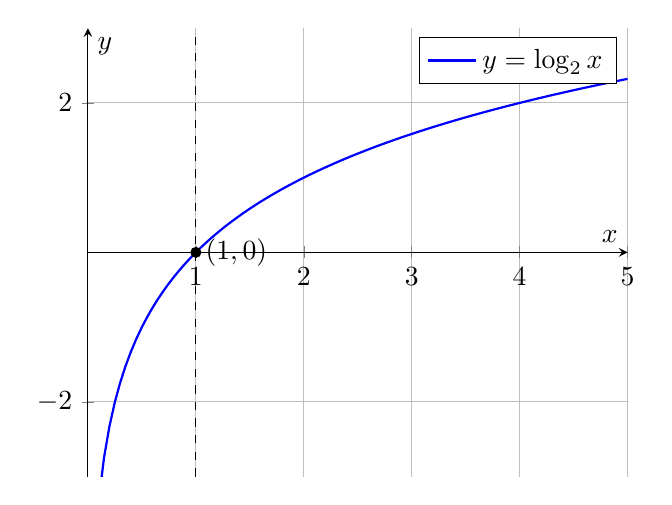
\begin{tikzpicture}
                \begin{axis}[
                    xmin=0, xmax=5,
                    ymin=-3, ymax=3,
                    axis lines=middle,
                    xlabel=$x$, ylabel=$y$,
                    grid=both,
                    samples=100,
                    domain=0.1:5
                ]
                \addplot[blue, thick] {ln(x)/ln(2)};
                \addlegendentry{$y=\log_2 x$};
                \draw[dashed] (1,-3) -- (1,3);
                \fill[black] (1,0) circle (2pt);
                \node[right] at (1,0) {$(1,0)$};
                \end{axis}
            \end{tikzpicture}
        \end{column}
    \end{columns}
  \end{frame}
  
  
  
  
  
  
  
  
  
  
  
  
  
  
  \begin{frame}{对数函数的图像与性质}
    \begin{columns}
        \begin{column}{0.5\textwidth}
            \begin{block}{当 $0 < a < 1$ 时}
                \begin{itemize}
                    \item 定义域:$(0, +\infty)$
                    \item 值域:$(-\infty, +\infty)$
                    \item 过定点 $(1, 0)$
                    \item 在 $(0, +\infty)$ 上单调递减
                \end{itemize}
            \end{block}
        \end{column}
        \begin{column}{0.5\textwidth}
            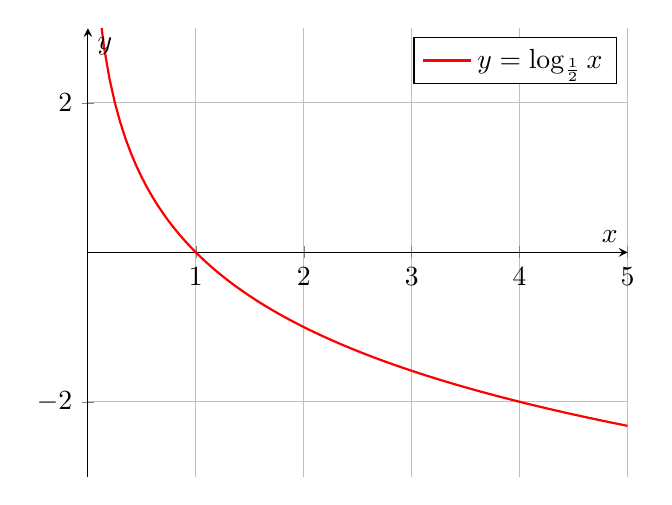
\begin{tikzpicture}
                \begin{axis}[
                    xmin=0, xmax=5,
                    ymin=-3, ymax=3,
                    axis lines=middle,
                    xlabel=$x$, ylabel=$y$,
                    grid=both,
                    samples=100,
                    domain=0.1:5
                ]
                \addplot[red, thick] {ln(x)/ln(0.5)};
                \addlegendentry{$y=\log_{\frac{1}{2}} x$};
                % \draw[dashed] (1,-3) -- (1,3);
                % \fill[black] (1,0) circle (2pt);
                % \node at (0,0) {$(1,0)$};
                \end{axis}
            \end{tikzpicture}
        \end{column}
    \end{columns}
  \end{frame}
  
  
  \begin{frame}{题目1:对数运算化简}
    \begin{block}{题目}
        化简下列表达式:
        \begin{enumerate}
            \item $\log_2 16 + \log_3 27$
            \item $\log_5 125 - \log_5 5$
            \item $\log_2 \sqrt{8} + \log_3 \frac{1}{9}$
        \end{enumerate}
    \end{block}
    
    \pause
    
    \begin{block}{答案}
        \begin{enumerate}
            \item $\log_2 16 + \log_3 27 = 4 + 3 = 7$
            \item $\log_5 125 - \log_5 5 = 3 - 1 = 2$
            \item $\log_2 \sqrt{8} + \log_3 \frac{1}{9} = \frac{3}{2} - 2 = -\frac{1}{2}$
        \end{enumerate}
    \end{block}
  \end{frame}
  
  
  
  \begin{frame}{题目2:对数方程求解}
    \begin{block}{题目}
        解下列方程:
        \begin{enumerate}
            \item $\log_3 x = 2$
            \item $\log_x 16 = 2$
            \item $\log_2 (x + 1) = 3$
        \end{enumerate}
    \end{block}
    
    \pause
    
    \begin{block}{答案}
        \begin{enumerate}
            \item $\log_3 x = 2 \implies x = 3^2 = 9$
            \item $\log_x 16 = 2 \implies x^2 = 16 \implies x = 4$($x > 0$且$x \neq 1$)
            \item $\log_2 (x + 1) = 3 \implies x + 1 = 2^3 \implies x = 7$
        \end{enumerate}
    \end{block}
  \end{frame}
  
  
  
  \begin{frame}{题目3:对数不等式求解}
    \begin{block}{题目}
        解不等式:
        \[
        \log_2 (x - 1) < 2
        \]
    \end{block}
    
    \pause
    
    \begin{block}{答案}
        \begin{enumerate}
            \item 定义域:$x - 1 > 0 \implies x > 1$
            \item 原不等式等价于:$\log_2 (x - 1) < \log_2 4$
            \item 由于底数 $2 > 1$,函数单调递增,故:
                  \[
                  x - 1 < 4 \implies x < 5
                  \]
            \item 结合定义域,解集为:$(1, 5)$
        \end{enumerate}
    \end{block}
  \end{frame}
  
  
  
  \begin{frame}{题目4:对数换底公式应用}
    \begin{block}{题目}
        计算:
        \[
        \log_2 3 \cdot \log_3 4 \cdot \log_4 5 \cdot \log_5 6 \cdot \log_6 7 \cdot \log_7 8
        \]
    \end{block}
    
    \pause
    
    \begin{block}{答案}
        \begin{enumerate}
            \item 利用换底公式:$\log_a b = \frac{\ln b}{\ln a}$
            \item 原式 $= \frac{\ln 3}{\ln 2} \cdot \frac{\ln 4}{\ln 3} \cdot \frac{\ln 5}{\ln 4} \cdot \frac{\ln 6}{\ln 5} \cdot \frac{\ln 7}{\ln 6} \cdot \frac{\ln 8}{\ln 7}$
            \item 约分后得:$\frac{\ln 8}{\ln 2} = \frac{3\ln 2}{\ln 2} = 3$
        \end{enumerate}
    \end{block}
  \end{frame}
  
  
  \begin{frame}{题目5:对数函数定义域与值域}
    \begin{block}{题目}
        求函数 $f(x) = \log_2 (x^2 - 4x + 3)$ 的定义域和值域。
    \end{block}
    
    \pause
    
    \begin{block}{答案}
        \begin{enumerate}
            \item 定义域:$x^2 - 4x + 3 > 0$
                  \[
                  (x - 1)(x - 3) > 0 \implies x < 1 \text{ 或 } x > 3
                  \]
            \item 令 $t = x^2 - 4x + 3$,则 $t$ 的取值范围为 $(0, +\infty)$
            \item 函数 $y = \log_2 t$ 的值域为 $(-\infty, +\infty)$
        \end{enumerate}
    \end{block}
  \end{frame}
  
  \begin{frame}[allowframebreaks]{题目6:对数函数定义域}
    \begin{block}{题目}
        求下列函数的定义域:
        \begin{enumerate}
            \item $f(x) = \log_3(2x - 5)$
            \item $g(x) = \ln(4 - x^2)$
            \item $h(x) = \log_{\frac{1}{2}}(x^2 - 2x - 3)$
            \item $k(x) = \frac{1}{\log_2(x - 1)}$
        \end{enumerate}
    \end{block}
    
    \pause
    
    \begin{block}{答案}
        \begin{enumerate}
            \item $2x - 5 > 0 \implies x > \frac{5}{2}$,定义域为$\left(\frac{5}{2}, +\infty\right)$
            \item $4 - x^2 > 0 \implies -2 < x < 2$,定义域为$(-2, 2)$
            \item $x^2 - 2x - 3 > 0 \implies (x - 3)(x + 1) > 0 \implies x < -1 \text{ 或 } x > 3$,定义域为$(-\infty, -1) \cup (3, +\infty)$
            \item $\begin{cases} x - 1 > 0 \\ \log_2(x - 1) \neq 0 \end{cases} \implies \begin{cases} x > 1 \\ x - 1 \neq 1 \end{cases} \implies x > 1 \text{ 且 } x \neq 2$,定义域为$(1, 2) \cup (2, +\infty)$
        \end{enumerate}
    \end{block}
  \end{frame}
  



\end{document}
